\section{Lecture 8, Stretch Reflex}
\subsection{Alpha motor neuron}
\begin{tabular}{p{4cm}p{15cm}}
Function	& $\alpha$-MN innervate skeletal muscle fibers and are directly responsible for their contraction.\\
Location	& They are mainly located in the spinal cord, except for $\alpha$-MN which control head and neck. In the spinal cord, $\alpha$-MNs are located in its gray matter.\\
Fine motor control	& The number of $\alpha$-MNs is directly proportional to the amount of fine control in a muscle.\\
Signaling	& The axons of $\alpha$-MNs are heavily myelinated and are large in diameter to ensure a high speed of the action potential propagation. Unlike most other neurons, $\alpha$-MNs use only acetylcholine as neurotransmitters.
\end{tabular}
\subsection{Stretch Reflex}
\begin{longtable}{p{4cm}p{15cm}}
		& 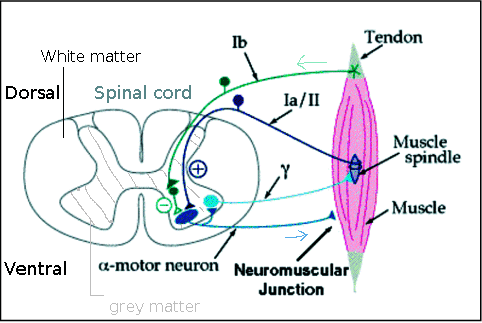
\includegraphics[width=12cm]{neuroinf_stretchreflex.png}\\
		& The stretch reflex is a monosynaptic process, since only a sensory neuron and a motor neuron are involved. There are about 620 muscles in a human body, and about 200 bones. Most of them are in our hands and feet.\\
Process		& \begin{enumerate}
		  	\item Muscle is stretched
			\item Muscle spindle is stretched and its nerve activity increases.
			\item $\alpha$ MN is activated, which causes the spindle to contract. Therefore, the length of the muscle fiber remains constant.
		  \end{enumerate}\\
Examples	& \begin{enumerate}
        	  	\item Leaning on a side
			\item Biceps reflex
			\item Knee-jerk reflex
        	  \end{enumerate}\\
Axon lengths	& \begin{tabular}[t]{ll}
		    White matter	& Grey matter\\\hline
		    4km / mm$^3$	& 9m / mm$^3$\\
		    Not myelinated	& Myelinated\\
		    Long distance, low bandwidth
		  \end{tabular}
\end{longtable}

